\documentclass[11pt]{article}
\usepackage{algorithm}
\usepackage{algpseudocode}
\usepackage{amssymb}
\usepackage[spanish]{babel}
\usepackage{graphicx}
\usepackage{hyperref}
\usepackage[utf8]{inputenc}
\usepackage{mathtools}
\usepackage{url}
\decimalpoint
\title{Desinfección mediante caminantes aleatorios}
\date{\today}
\author{Aldo Sayeg Pasos Trejo}
\begin{document}
\maketitle
\tableofcontents
\section{Simulacion de desinfección}
La simulación que realizamos puede primero describirse en términos más simples mediante el siguiente algoritmo:
\begin{algorithm}[h]
    \caption{Simulacion de desinfeccion}
    \begin{algorithmic}[1]
    \Function{Desinfección}{$n_g$,$n_v$,$t_s$,RadioDecrece}
        \State Genera posiciones iniciales para $n_v$ particulas de virus
        \State Genera posiciones iniciales para $n_g$ particulas de gel 
        \For{$i = 1,\ldots,t_s$}
            \For{$j = 1,\ldots,n_g$}
                \State Avanza la $j$-ésima partícula de gel en una dirección aleatoria
                \State Checa cuantas de las $n_v$ partículas de virus están a distancia $r_j$ de la $j$-ésima partícula de gel. 
                \State Aumenta el número de visitas la partículas de virus que estén dentro del radio $r_j$
                \If{RadioDecrece}
                    \State Disminuye $r_j$
                \EndIf 
            \EndFor
        \EndFor
    \EndFunction
    \end{algorithmic}
\end{algorithm}
\section{Posiciones del virus como resultado de la simulación de un estornudo}
Las posiciones iniciales del virus se generan a través de la solución a un sistema de ecuaciones diferenciales, correspondiente al tiro parabólico en 3D con fricción lineal en la velocidad. Explícitamente, el sistema de ecuaciones es:
\begin{equation}
    \begin{dcases}
        \label{tiroParab}
        \ddot{x}+ \frac{3\pi D \mu}{6} \dot{x} = 0  \\ 
        \ddot{y}+\frac{3\pi D \mu}{6} \dot{y} = 0  \\ 
        \ddot{z}+\frac{3\pi D \mu}{6} \dot{z} + g = 0  \\ 
    \end{dcases}
\end{equation}
Las condiciones iniciales para el sistema de EDOs corresponden a
\begin{equation}
    \begin{gathered}
        \label{tiroParabCI}
        (x,y,z) = (0,0,h) \\
        (\dot{x},\dot{y},\dot{z}) = (R\sin(\Theta)\cos(\Phi),R\sin(\Theta)\sin(\Phi),R\cos(\Theta))
    \end{gathered}        
\end{equation}
con $h$ la altura de una persona que queramos simular, $R$ (la magnitud de la velocidad inicial) es una variable aleatoria tomada uniformemente en el intervalo $[2,3]$, $\Theta$ el angulo polar tomado uniformemente en el intervalo $[\pi/8,\pi/4]$ y $\Phi$ es el angulo azimutal, tomado uniformemente en el intervalo  $[-\pi/4,\pi/4]$.
\\
\\Para obtener la posición inicial de una partícula de virus, resolvemos el sistema \ref{tiroParab} con condiciones iniciales $\ref{tiroParabCI}$. La posición inicial es el valor $(y(t^*),z(t^*))$ donde $t^*$ es el primer tiempo discreto a partir del cual $x(t^*) > 1.0$ y $z(t^*) > 0.5$
\section{Caminantes aleatorios y movimiento browniniano}
Una variable aleatoria es una función $X:\Omega \to \mathbb{R}$. En palabras simples, es un posible número real que toma uno de varios valores posibles (inclusive una infinidad), cada uno con distinta probabilidad. Ejemplos de variables aleatorias son:
\begin{itemize}
    \item El resultado de tirar un dado.
    \item El resultado de tirar un volado codificamos si ``águila'' como $0$ y ``sol'' como $1$.
    \item El resultado de tomar un punto al azar en un círculo.
    \item El resultado de tomar un punto al azar en una recta.
\end{itemize}
Una cosa importante que deben distinguir es que la variable aleatoria es el posible número con todos sus valores, no es el resultado en sí. Un ejemplo sencillo es el siguiente: si tiran un dado y cae un número 6, el número 6 \textbf{no es un variable aleatoria}, la variable aleatoria es \textbf{el posible resultado de tirar un dado}. Número 6, es decir, al resultado en sí de tirar el dado, le decimos \textbf{muestra} de la variable aleatoria de tirar el dado.
\\
\\Cuando tenemos muchas variables aleatorias $X_1,X_2,\ldots $, es decir, tenemos un conjunto $\{X_n \mid n \in \mathbb{N}\}$, decimos que tenemos un \textbf{proceso estocástico}. Ya que $n \in \mathbb{N}$, en particular decimos que tenemos un proceso estocástico \textbf{a tiempo discreto} o a pasos discretos. Uno de los procesos estocásticos más sencillos es la \textbf{caminata aleatoria 1D}. Una caminata aleatoria 1D se define de forma recursiva como:
\begin{equation}
    \begin{gathered}
        X_0 = 0 \\
        X_n = \begin{dcases}
            X_{n-1}+1 & \text{con probabilidad } 1/2 \\
            X_{n-1}-1 & \text{con probabilidad } 1/2 \\
        \end{dcases}
    \end{gathered}
\end{equation}
La siguiente figura ilustra un conjunto de 10 caminatas aleatorias independientes.
\begin{figure}[h]
    \centering
    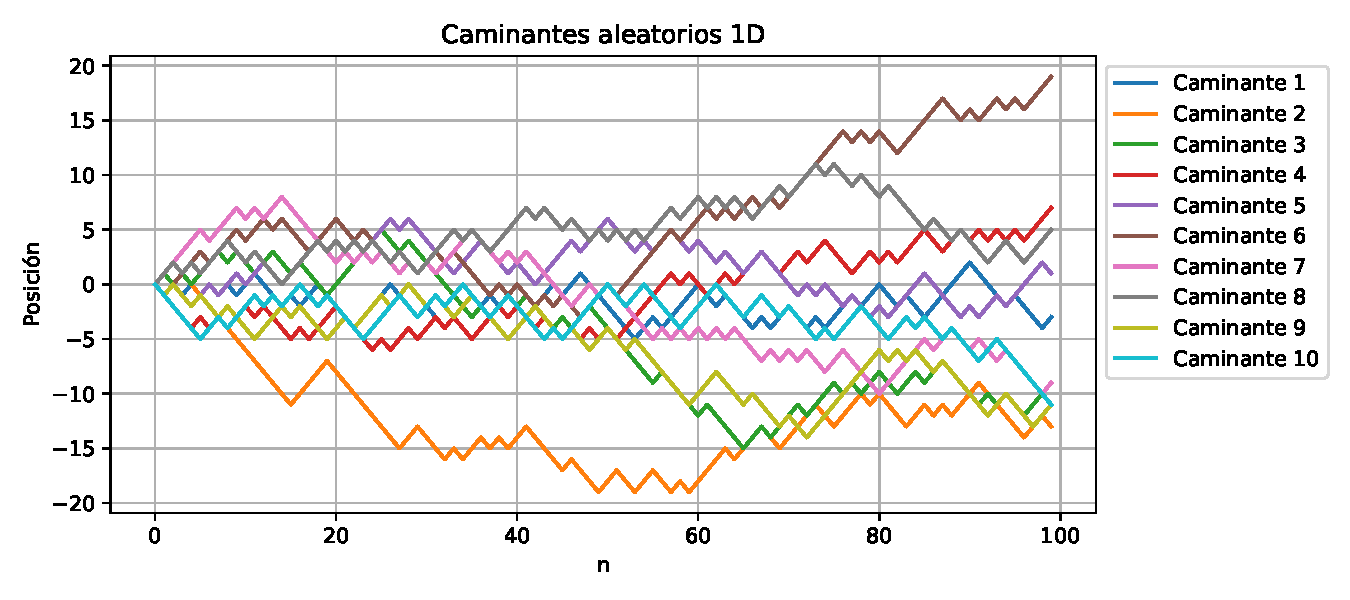
\includegraphics[width=\textwidth]{caminantes.pdf}
    \caption{10 caminantes aleatorios independientes}
\end{figure}
En general, no es importante que el punto inicial de una caminata aleatoria sea 0. Basta con que sea un punto constante cualquiera. La caminata aleatoria se puede extender de forma trivial a varias dimensiones. Aunque hay distintas formas de extenderla, nosotros en la simulación hacemos una caminata aleatoria en $\mathbb{R}^2$ de la siguiente forma: 
\begin{itemize}
    \item El punto inicial es un punto $(X_0,Y_0)$ escogido al azar de forma uniforme en el rectángulo más pequeño que contiene a todas las partículas de virus.
    \item En cada paso, hacemos $(X_{n+1},Y_{n+1}) = (X_n,Y_n) + (R\cos(\Theta),R\sin(\Theta))$ donde $R$ es una variable aleatoria uniforme en el intervalo $[0,0.05]$ y $\Theta$ un ángulo aleatorio en el intervalo $[0,2\pi)$
\end{itemize}
\section{Búsquedas de vecinos: árboles KD}
En cada paso de la simulación se realiza el siguiente procedimiento: para cada partícula de gel, con un radio dado $r$, buscamos cuántas partículas de virus se encuentran a una distancia $r$ de ella. Si tenemos $n_g$ partículas de gel y $n_v$ partículas de virus, entonces necesitaríamos realizar $n_g \times n_v$ operaciones de búsqueda para contabilizar cuántas de las $n_v$ partículas de virus están en contacto con las $m_g$ partículas de gel. 
\\
\\Sin embargo, podemos resolver esto de forma más rápida si en lugar de buscar si cada partícula de virus está en el radio de cada partícula de gel, utilizamos un árbol KD \cite{kdtrees} sobre las posiciones de los viruses para poder buscar entonces, dada una particula de gel y su radio, todas las partículas de virus a una distancia menor a $r$ de la partícula de gel.
\\
\\Un árbol KD es una \textbf{estructura de datos} (una forma ingeniosa de representar información en una computadora) que permite, dado un conjunto fijo de $n$ puntos en $\mathbb{R}^d$, buscar los puntos más cercanos a otro. La estructura permite que encontremos todos el punto más cercano del conjunto a cualquier otro con tan solo $ \log(n)$ operaciones, a diferencia de las usuales $n$.
\section{Consideraciones extra}
\begin{itemize}
    \item Para darle más realismo, una posibilidad es tomar los radios no iguales para todas las partículas de gel si no muestrear los radios de una variable aleatoria normal (gaussiana) con promedio distinto de 0. En las animaciones, el radio promedio es 0.05. 
    \item También es posible, en una metáfora directa con la evaporación del alcohol, hacer una simulación en la cuál los radios de las partículas se reduzcan linealmente hasta volverse 0 en el paso final de la simulación.
    \item Las partículas de virus pueden tener distintos perfiles de vitalidad, es decir, la forma en la que dejan de funcionar como función del número de visitas de partículas de gel que han tenido. La figura \ref{fig:vitalidad} muestra perfiles exponenciales, lineales y logarítmos para la vitalidad de las partículas.
    \begin{figure}[h]
        \centering
        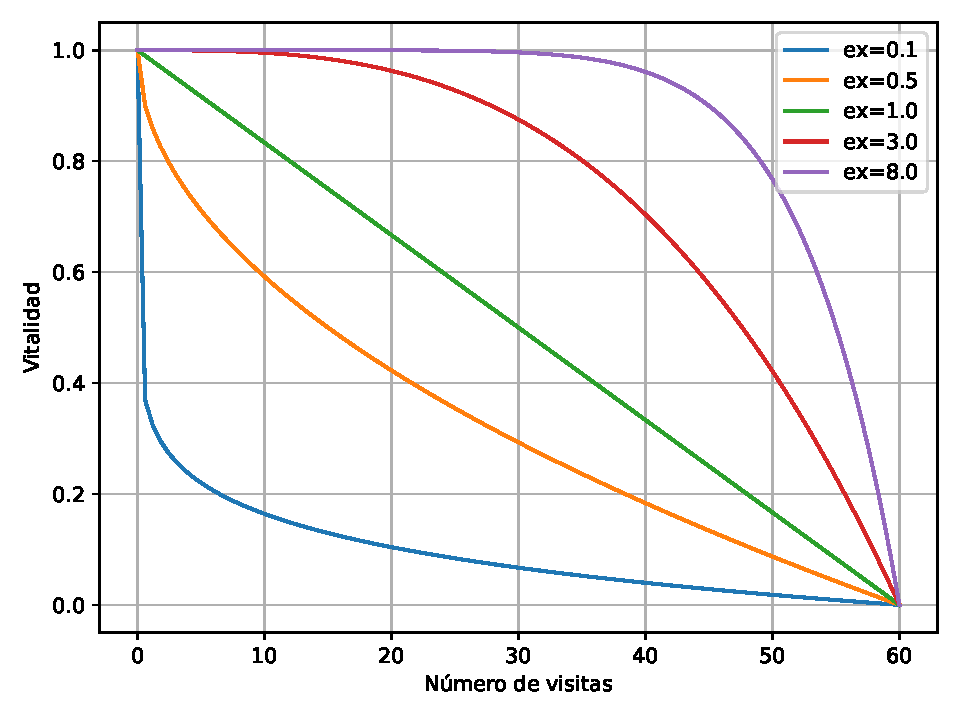
\includegraphics[width=\textwidth]{vitalidad.pdf}
        \caption{Distintos perfiles de vitalidad para las partículas de virus. En todos los casos, los virus mueren cuando son visitados 60 veces}
        \label{fig:vitalidad}
    \end{figure}
\end{itemize}
\section{Simulación revisada}
Con toda la información que acabamos de mencionar, podemos volver a escribir el código de la simulación. 
\begin{algorithm}[h]
    \caption{Simulacion de desinfeccion}
    \begin{algorithmic}[1]
    \Function{Desinfección}{$n_g$,$n_v$,$t_s$,RadioDecrece}
        \State General posiciones iniciales para $n_v$ particulas de virus resolviendo la ecuación diferencial \ref{tiroParab}.
        \State Crea un árbol KD con las posiciones de las $n_v$ partículas.
        \State General posiciones iniciales para $n_g$ particulas de gel en el rectángulo mínmimo que contiene a todas las $n_v$ partículas.
        \For{$i = 1,\ldots,t_s$}
            \For{$j = 1,\ldots,n_g$}
                \State Avanza la $j$-ésima partícula de gel en una dirección aleatoria.
                \State Usa el árbol kd para checar cuantas de las $n_v$ partículas de virus están a distancia $r_j$ de la $j$-ésima partícula de gel. 
                \State Aumenta el número de visitas la partículas de virus que estén dentro del radio $r_j$
                \If{RadioDecrece}
                    \State Disminuye $r_j$ para que se vuelva cero cuando $i = ts$
                \EndIf 
            \EndFor
        \EndFor
    \EndFunction
    \end{algorithmic}
\end{algorithm}
\begin{thebibliography}{9}
    \bibitem{kdtrees}
      Árbol kd - Wikipedia, la Enciclopedia Libre.
      \url{https://es.wikipedia.org/wiki/%C3%81rbol_kd}. Accesado el 25-09-2021
\end{thebibliography}
\end{document}
